\lab{Optimization with Scipy}{scipy.optimize}
\label{lab:Optimization1}
\objective{Introduce some of the basic optimization functions available in \li{scipy.optimize}}

The Optimize package in Scipy has several functions for minimizing, root finding, and curve fitting. Here we will cover the usage of many of these functions.
You can learn about all of the functions at \url{http://docs.scipy.org/doc/scipy/reference/optimize.html}.

\section*{Local Minimization}

First we will test out a few of the minimization algorithms on the Rosenbrock Function, which is defined as
\[
f(x,y) = (1-x)^2 + 100(y-x^2)^2.
\]
The Rosenbrock function is commonly used when evaluating the performance of an optimization algorithm.
Reasons for this include the fact that its minimizer \li{x = np.array([1., 1.])} is found in  curved valley, and so minimizing the function is non-trivial.
See Figure \ref{opt:rosenbrock}.
The Rosenbrock function is included in the optimize package (as \li{rosen}), as well as its gradient (\li{rosen_der}) and its hessian (\li{rosen_hess}).

\begin{figure}
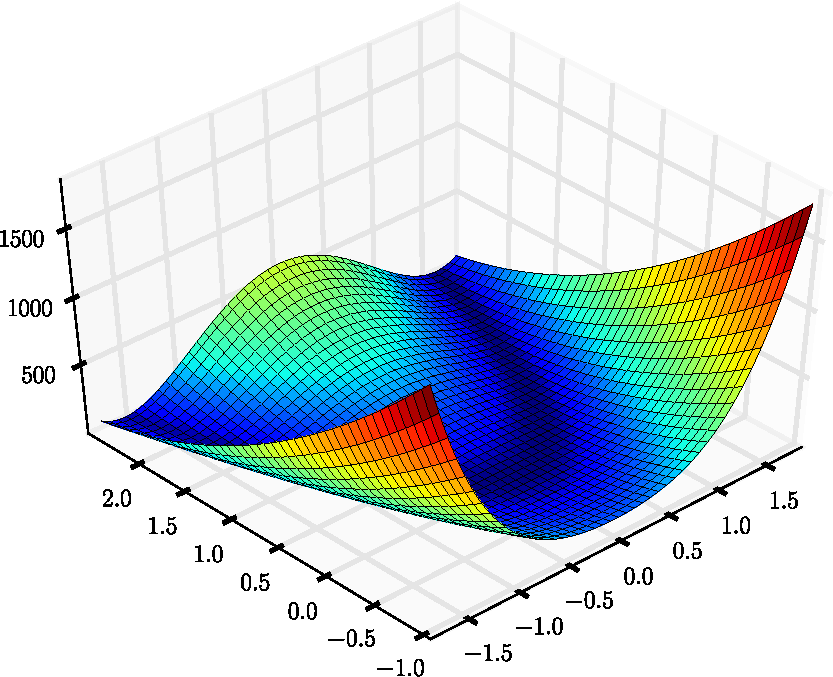
\includegraphics[width=\textwidth]{Rosenbrock.pdf}
\caption{$f(x,y) = (1-x)^2 + 100(y-x^2)^2$}
\label{opt:rosenbrock}
\end{figure}

We will use the \li{minimize()} function and test each of its algorithms (specified by the keyword argument ``method" -- see the documentation page for \li{minimize()}).
Note that there are also several functions such as \li{fmin} and \li{fmin_powell}. These are equivalent to using the \li{minimize()} function with the specified method.

For each algorithm, you need to pass in a callable function object for the Rosenbrock function, as well as a NumPy array giving the initial guess.
For some algorithms, you will additionally need to pass in the jacobian or hessian.
You may recognize some of these algorithms, and several of them will be discussed in greater detail later. For this lab, you do not need to understand how they work, just
how to use them.

% Here give an example (Change so not Nelder-Mead) and expalin how to read the output
As an example, we'll minimize the Rosenbrock with the Newton-CG method. This method often performs better by including the optional hessian as an argument, which we will do here.
\begin{lstlisting}
>>> import numpy as np
>>> from scipy import optimize as opt
>>> x0 = np.array([4., -2.5])
>>> opt.minimize(opt.rosen, x0, method='Newton-CG', hess=opt.rosen_hess, 
													jac=opt.rosen_der)
     fun: 1.1496545381999877e-15
     jac: array([  1.12295570e-05,  -5.63744647e-06])
 message: 'Optimization terminated successfully.'
    nfev: 45
    nhev: 34
     nit: 34
    njev: 78
  status: 0
 success: True
       x: array([ 0.99999997,  0.99999993])
\end{lstlisting}
As the online documentation indicates, \li{opt.minimize()} returns an object of type \li{opt.optimize.OptimizeResult}. 

The printed output gives you information on the performance of the algorithm. 
The most relevant output for this lab include 

\li{fun: 1.1496545381999877e-15}, the obtained minimum; 

\li{nit: 96}, the number of iterations the algorithm took to complete; 

\li{success: True}, whether the algorithm converged or not; 

\li{x: array([ 0.99999997,  0.99999993])}, the obtained minimizer.

Each of these outputs can be accessed either by indexing \li{OptimizeResult} object like a dictionary (\li{result['nit']}), or as attributes of a class (\li{result.nit}).  We recommend access by indexing, as this is consistent with other optimization packages in Python.

The online documenation for \li{scipy.optimize.minimize()} includes other optional parameters available to users, for example, to set a tolerance of convergence. While these are not required for this lab, they should be explored as needed for specific applications.

\begin{problem}
Use the \li{opt.minimize()} function to find the minimum of the Rosenbrock function.
Test Nelder-Mead, CG, and BFGS, starting each with the initial guess \li{x_0 = np.array([4., -2.5])}.
For each method, print whether it converged, and if so, print how many iterations it took.

Note that the hessian argument is not needed for these paticular methods. 
\end{problem}

Each of these three algorithms will be explored in great detail later in Volume 2: Nelder-Mead is a variation of the Simplex algorithm, CG is a variant of the Conjugate Gradient algorithm, and BFGS is a quasi-Newton method developed by Broyden, Fletcher, Goldfarb, and Shanno.

\section*{Global Minimization via Basin Hopping}

In the realm of optimization, convex functions are the most well-behaved, as any local minimum is a global minimum.
However, in practice one must frequently deal with non-convex functions, and sometimes we need pick the global minimum out of many local minima.

For example, consider the function
%This is the crazy function that I came up with to stump the algorithms
\[
z = r^2 (1+ \sin^2(4r)),
\]
where
\[
r = \sqrt{(x+1)^2 + y^2}.
\]
Essentially, this is a wavy crater offset from the origin by 1 along the $x$ axis (see Figure \ref{opt:multimin}).
\begin{figure}
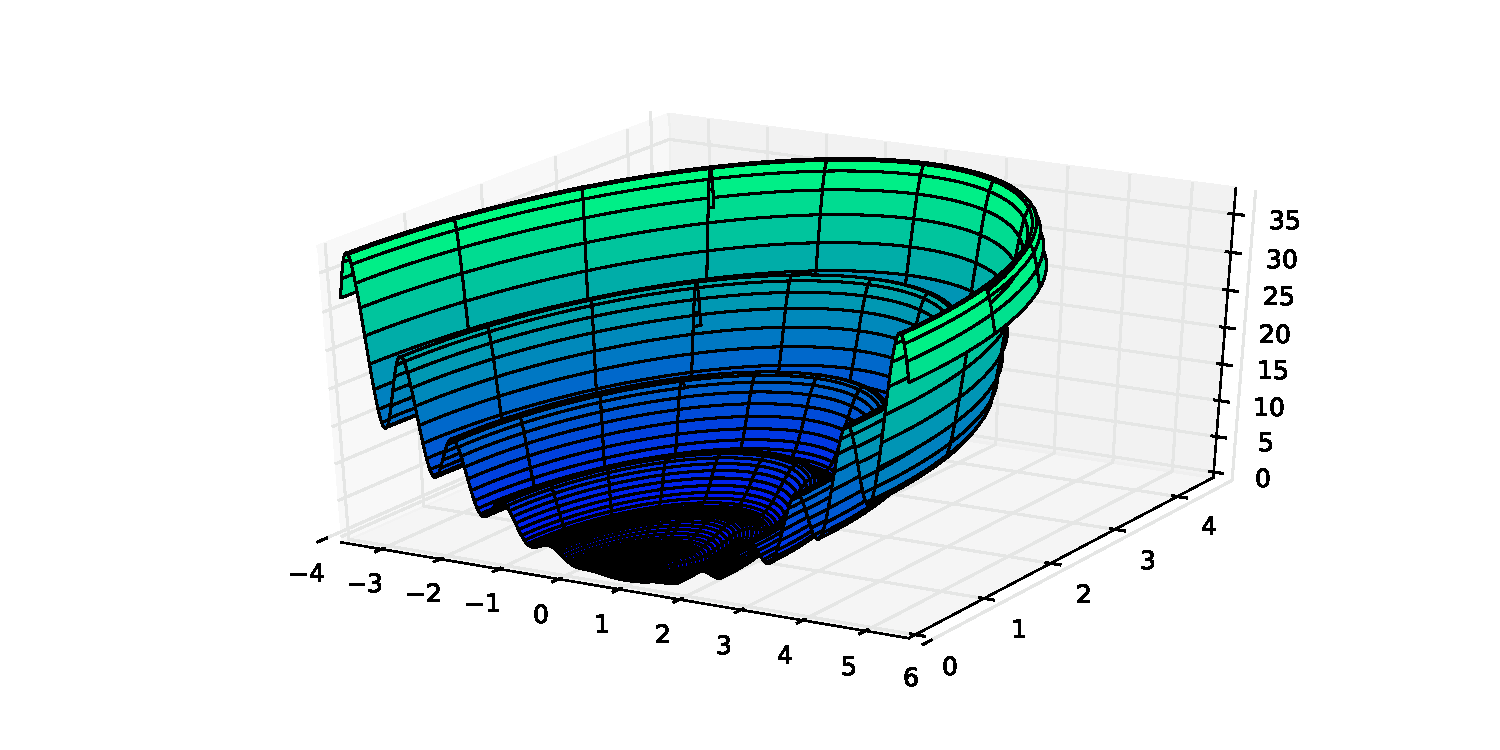
\includegraphics[width=\textwidth]{ManyMinima.pdf}
\caption{$z = r^2 (1+ 2\sin^2(4r))$}
\label{opt:multimin}
\end{figure}
The presence of many local minima proves to be a difficulty for the minimization algorithms.

For example, if we try using the Nelder-Mead method as previously, with an initial point of \li{x0 = np.array([-2, -2])}, the algorithm fails to find the global minimum, and instead comes to rest on a local minimum.
\begin{lstlisting}
>>> def multimin(x):
>>>     r = np.sqrt((x[0]+1)**2 + x[1]**2)
>>>     return r**2 *(1+ np.sin(4*r)**2)
>>>
>>> x0 = np.array([-2, -2])
>>> res = opt.minimize(multimin, x0, method='Nelder-Mead')
 final_simplex: (array([[-2.11758025, -2.04313668], [-2.11748198, -2.04319043],
       [-2.11751491, -2.04317242]]), array([ 5.48816866,  
       												5.48816866,  5.48816866]))
           fun: 5.488168656962328
       message: 'Optimization terminated successfully.'
          nfev: 84
           nit: 44
        status: 0
       success: True
             x: array([-2.11758025, -2.04313668])
>>> print res['x']
[-2.11758025, -2.04313668]
>>> print res['fun']
5.488168656962328
>>> print multimin([-1,0])
0.0
\end{lstlisting}

However, SciPy does have some tools to help us with these problems. Specifically, we can use the \li{opt.basinhopping()} function.
Conceptually, most of the minimizing algorithms use the derivative of the function to search in a downhill direction for potential minimizers.
Often they overshoot the minimum and later backtrack. You can think of it as a ball rolling down a hill into a valley.
At first, the momentum of the ball carries it across the valley floor and partially up the other wall, only to roll back into the valley.
Slowly the ball loses momentum as it repeatedly overshoots and backtracks. Eventually the ball comes to rest at the bottom of a valley -- hopefully the lowest valley.
However, if there are many valleys (or local minima), the ball can get stuck in one that's not the lowest.
The \li{opt.basinhopping()} function uses the same minimizing algorithms (in fact, you can tell it whatever minimizing algorithm you can pass to \li{opt.minimize()}).
However, once it settles on a minimum, it hops to a new point in the domain (depending on how we set the ``hopping" distance) that hopefully lies outside of the valley
or basin belonging to the current local minimum.
It then searches for the minimum from this new starting point, and if it finds a better minimizer, it repeats the hopping process from this new minimizer.

\emph{Only Scipy Version 0.12+ has \li{opt.basinhopping}. In earlier versions, such as 0.11, you won't find it.}

\begin{problem}
Explore the documentation for the \li{opt.basinhopping()} function online or via IPython, 
and use it to find the global minimum of our \li{multimin()} function with \li{x0 = np.array([-2, -2])}.
Call it using the same \li{Nelder-Mead} algorithm with \li{opt.basinhopping(multimin, x0, stepsize=0.5, minimizer_kwargs=\{'method':'nelder-mead'\})}.
Try it first with \li{stepsize=0.5} and then with \li{stepsize=0.2}. 

Plot the multimin function using the following code:
\begin{lstlisting}
>>> xdomain = np.linspace(-3.5,1.5,70)
>>> ydomain = np.linspace(-2.5,2.5,60)
>>> X,Y = np.meshgrid(xdomain,ydomain)
>>> Z = multimin((X,Y))
>>> fig = plt.figure()
>>> ax1 = fig.add_subplot(111, projection='3d')
>>> ax1.plot_wireframe(X, Y, Z, linewidth=.5, color='c')
\end{lstlisting}

Plot the initial point and minima by adapting the following line:
\begin{lstlisting}
>>> ax1.scatter(x_value, y_value, z_value)     
\end{lstlisting}

Why doesn't the alogrithm find the global minimum with \li{stepsize=0.2}?
Print your answer to this question, and return the true global minimum.
\end{problem}

\section*{Root Finding}

The \li{optimize} package also has functions useful in root-finding.
The next example, taken from the online documentation, solves the following nonlinear system of equations using \li{opt.root}.

\[
\begin{bmatrix}
	x_{0} + 1/2 ( x_{0} - x_{1} )^{3} - 1 \\
	1/2(x_{1}-x_{0})^{3} + x_{1}
\end{bmatrix} =
\begin{bmatrix}
	0 \\
	0
\end{bmatrix}.
\]

\begin{lstlisting}
>>> def func(x):
>>>     return [x[0] + 0.5 * (x[0] - x[1])**3 -1.0,
>>>             0.5 * ( x[1] - x[0])**3 + x[1]]
>>> def jac(x):
>>>     return np.array([[1 + 1.5 * (x[0] - x[1])**2,
>>>                     -1.5 * (x[0] - x[1])**2],
>>>                     [-1.5 * (x[1] - x[0])**2,
>>>                     1 + 1.5 * (x[1] - x[0])**2]])
>>> sol = opt.root(func, [0, 0], jac=jac, method='hybr')
>>> print sol.x
[ 0.8411639  0.1588361]
>>> print func(sol.x)
[-1.1102230246251565e-16, 0.0]
\end{lstlisting}

\begin{problem}
Find the roots of the system
\[
\begin{bmatrix}
	-x+y+z \\
	1+x^3-y^2+z^3\\
	-2-x^2+y^2+z^2
\end{bmatrix} =
\begin{bmatrix}
	0 \\
	0 \\
	0
\end{bmatrix} .
\]
Return the values of $x,y,z$ as an array.
\end{problem}



As with \li{opt.minimize()}, \li{opt.root()} has more than one algorithm for root finding.
Here we have used the \li{hybr} method. There are also several algorithms for scalar root finding. See the online documentation for more.

\section*{Curve Fitting}

%we still have curve fitting
%least squares programming -- but it seems that it's already been done in Volume One

SciPy also has methods for curve fitting wrapped by the \li{opt.curve_fit()} function.
Just pass it data and a function to be fit. The function should take in the independent variable as its first argument and
values for the fitting parameters as subsequent arguments.
Examine the following example from the online documentation.
\begin{lstlisting}
>>> import numpy as np
>>> import scipy.optimize as opt

>>> #the function with which to create the data and later fit it
>>> def func(x,a,b,c):
>>>     return a*np.exp(-b*x) + c

>>> #create perturbed data
>>> x = np.linspace(0,4,50)
>>> y = func(x,2.5,1.3,0.5)
>>> yn = y + 0.2*np.random.normal(size=len(x));

>>> #perform the fit
>>> popt, pcov = opt.curve_fit(func,x,yn)
\end{lstlisting}
The variable \li{popt} now contains the fitted parameters and \li{pcov} gives the covariance of the fit.
See Figure \ref{opt:curve_fit} for a plot of the data and the fitted curve.

\begin{figure}
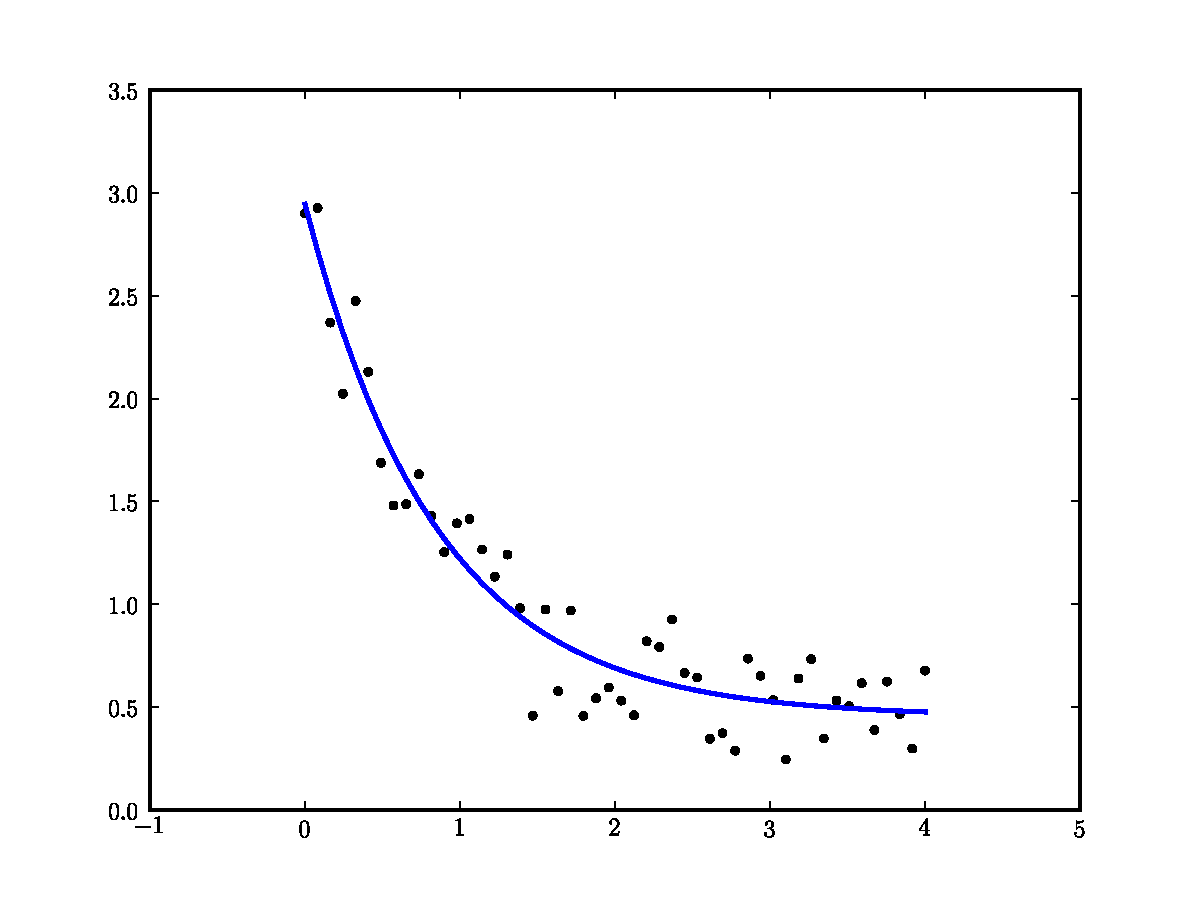
\includegraphics[width=\textwidth]{curve_fit.pdf}
\caption{Perturbed data graphed with the curve using the fitted parameters: $a=2.72$,  $b=1.31$, and $c=0.45$.}
\label{opt:curve_fit}
\end{figure}

\begin{problem}
Use the \li{opt.curve_fit} function to fit a curve to data obtained from numerical simulations of convection.
The data are in the file \li{convection.npy}. The first column is $R$, the Raleigh number, and the second column is $\nu$.
The relevant convection equation is:
\[
\nu = cR^\beta,
\]
where $\nu$ is nu, $R$ is the Raleigh number, $c$ is some constant, and $\beta$ is another constant. 
Use \li{opt.curve_fit()} to find a fit to the data using $c$, and $\beta$ as the fitting parameters.
Just so that you know that you are getting realistic values, $c$ should be on the order of $10^{-2}$, and $\beta$ on the order of $10^{0}$.
Return your values for $c$, and $\beta$ in a NumPy array of length 2.

See Figure \ref{opt:ConvectionFit} for a plot of the data along with a fitted curve.
\end{problem}

\begin{figure}
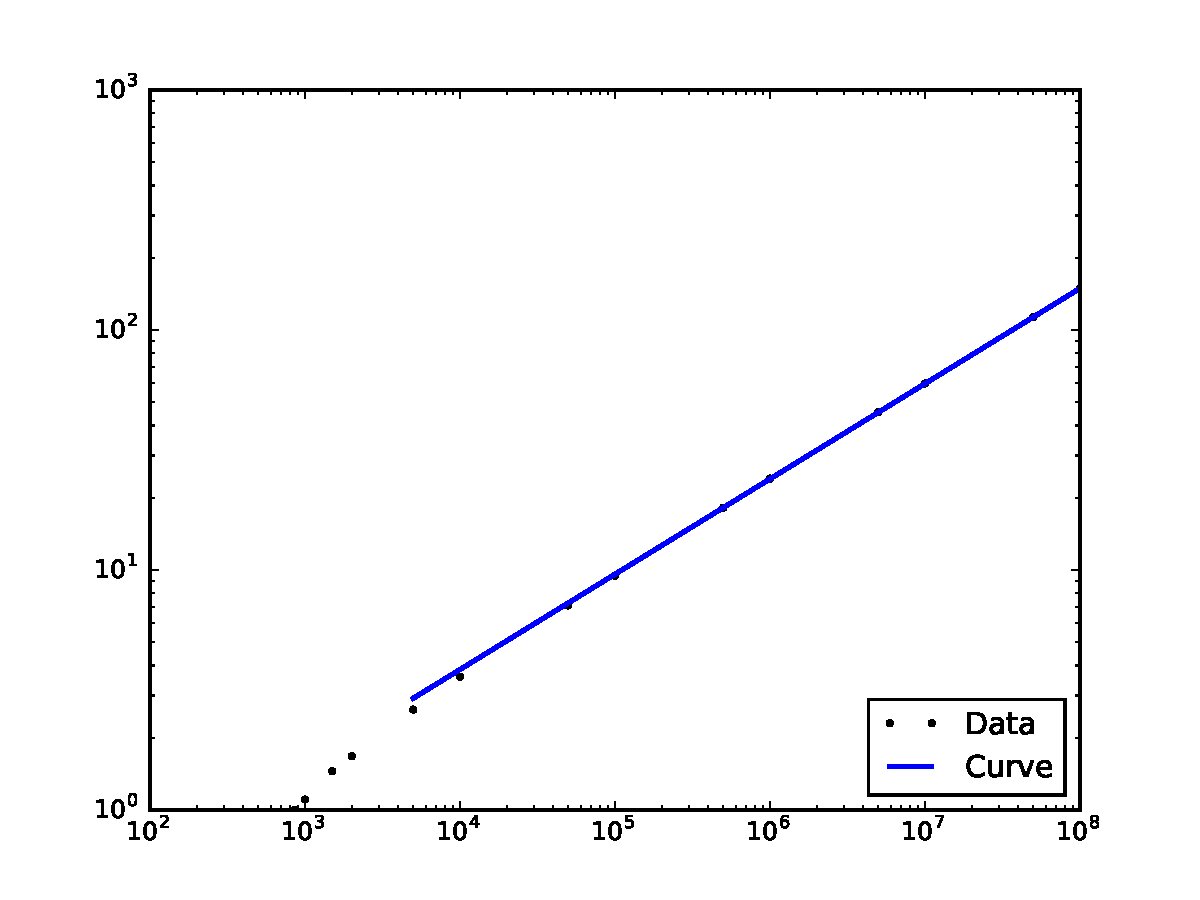
\includegraphics[width=\textwidth]{ConvectionFit.pdf}
\caption{The black points are the data from \li{convection.npy} plotted as a scatter plot. The blue line is a fitted curve.}
\label{opt:ConvectionFit}
\end{figure}

The \li{scipy.optimize} package has many other useful functions, and is a good first resource when confronting a numerical optimization problem. See the online documentation for further details.


